\chapter{Perspektivering - Affjedring af biler}
Den harmoniske svingning optræder mange andre steder i mekanikken, end bare når et lod svinger i en fjeder.
Den ses blandt andet i forbindelse med penduler og generelt med ting, der drejer rundt.
Derudover er det også relevant at kigge på i forbindelse med større bygninger, eksempelvis broer, der kan gå i svingninger hvis de ikke er konstrueret rigtigt. 

Et andet sted hvor man kan se svingninger af fjedre meget markant, er i forbindelse med affjedring af biler. 
Det er nemlig sådan at en bils hjul er forbundet til fjedre. 
En skitse af dette kan ses på figur \ref{fig: Affjedring af bil}.

\begin{wrapfigure}{r}{0.4\textwidth}
\center
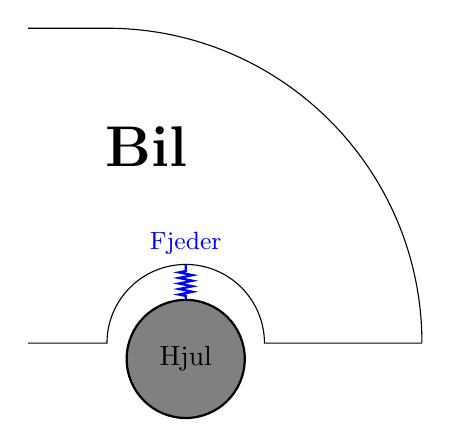
\begin{tikzpicture}
\tikzstyle{spring}=[thick,decorate,decoration={zigzag,pre length=0.05cm,post length=0.05cm,segment length=2}]

\draw (-2,0)--(-1,0)--(-1,0) arc [radius=1, start angle=180, end angle= 0]--(1,0)--(3,0);%Bund af bil uden hjul

\draw (3,0) arc [radius=4, start angle=0, end angle = 90] -- (-2,4) ;%Top af bil

\draw[fill=gray, thick] (0,-0.2) circle (0.75) node {Hjul};%hjulet
\node at (-0.5,2.5) {\huge \textbf{Bil}};
\draw[spring, blue] (0,0.55)--(0,1) node[above, blue] {\small Fjeder};

\end{tikzpicture}
\caption{Skitsetegning af fjeder (blå) fastsat til bils hjul.}
\label{fig: Affjedring af bil}
\end{wrapfigure}

Fjederen er til for at sørge for, at bilen hele tiden fastholder kontakt med vejen - også selvom den kører over en ujævnhed. 
Hvis fjederen går i stykker, kan det være meget problematisk. 
Der kan ske det, at fjederen dæmper for langsomt, og at man derfor oplever at bilen hopper.
En video af af dette kan ses på YouTube\refBilVideo.
På videoen ser vi en mand, der trykker på forenden af sin bil. 
Når han giver slip, står bilen og svinger op og ned. 
Hvis man betragter denne svingning med den teori, der er beskrevet i denne opgave, så svarer bilen til vores lod.
Vi er da interesserede i at få svingningen af bilen til at dø ud så hurtigt som muligt. 
Her arbejder vi ikke med luftmodstand, men derimod med en mekanisk dæmpning. 
Hvis vi antager, at svingningen dæmpes på en måde, således at dæmpningen er proportional med hastigheden af svingningen med en proportionalitetskonstant $\xi$, har vi igen en lineær andenordens homogen differentialligning

$$mx''(t)+\xi x'(t) + k x(t) = 0$$

hvor $k$ er fjederkonstanten for bilens fjeder, $m$ er bilens masse, og $x$ er en funktion af tiden, der beskriver, hvor højt/lavt bilen befinder sig i forhold til sit udgangspunkt.

Da vi er interesserede i, at bilen hopper så lidt som muligt, er vi ikke interesserede i en harmonisk svingning. 
Vi ved fra teorien tidligere, at der opstår en harmonisk svingning, når rødderne i karakterligningen er komplekse. 
Derfor er man interesseret i at få en god nok kombination af dæmpningskonstant og fjederkonstant til, at rødderne i karakterligningen ikke bliver komplekse. 

Vi vil derfor gerne prøve at kigge på karakterligningen. 
Vi får da en ligning $mr^2 + \xi r + k = 0$ hvilket giver os løsningerne (med andengradslignings løsningsformel):

$$r = \dfrac{-\xi \pm \sqrt{\xi ^2 - 4mk}}{2m}$$

For at vi ikke får komplekse rødder, skal vi altså have, at størrelsen $\xi ^2 -4mk$ er ikke-negativ, og det skal altså gælde at $0 \leq \xi ^2 -4mk $ eller omskrevet at $4mk \leq \xi ^2 $.
Her fra er man dog nødt til at vide mere omkring biler og kunne foretage nogle eksperimenter for at kunne fortsætte. 
Vi ved nemlig intet om $\xi$, og om hvordan dæmpning skabes. 

I forhold til videoen, kan vi se at bilen lige pludselig svinger, og at karakterligningen derfor må have komplekse løsninger.
Vi ved derfor, at der er sket en ændring af $k,m$ og $\xi$ sådan, at det ikke længere gælder, at $4mk \leq \xi ^2 $.
Da bilens masse, $m$, formentlig ikke har ændret sig, må vi altså enten have at $k$ er blevet større eller at $\xi$ er blevet mindre. 
Oversat til fysik, har vi altså enten, at fjederen er blevet mere hård og derfor har en højere fjederkonstant, eller at dæmpningssystemet ikke fungerer som det skal.

\vspace{0.75cm}

Bemærk, at dette ikke på nogen måde er baseret eksperimentelt    på biler, men bare er et forsøg på at overføre min model fra loddet til en bil. 
Det er mange ting, der bør tages højde for, som denne perspektivering ikke kigger på.
Dog kan det ses at modellen, som der er fundet frem til i denne opgave, ikke er irrelevant til at beskrive andre fysiske fænomener.

